\section{Base Station}
The original design for the base station called for a self-contained Linux
system to collect and process the measurements from the other PICA
systems. To accomplish this goal, the design team decided to use an
\ac{FPGA} development board and program it will the SPARC-compatible LEON3
soft-processor, which is licensed under the \ac{GPL}. While this option
showed a great deal of promise, it ultimately lead to more obstacles than
the team decided could be overcome without detracting from the other areas
of the project. In light of this decision, the role of the base station
will be fulfilled by a standard desktop computer using custom software to
perform the tasks that an embedded system would have performed.


%\begin{figure}[htbp]
%\begin{center}
%\includegraphics[width=5in]{includes/}
%\caption{Base Station functional block diagram}
%\label{fig:base_station_block_diagram}
%\end{center}
%\end{figure}

\subsection{Device Selection}
%TODO: Distinguish between GRlib peripherals and the LEON3 processor
One of the key factors in creating an embedded system is determining the
processing power required. As most of the devices connected to the base
station aggregate their own data and send only summaries to the base
station, the base station does not require a lot of processing power. It
does, however, need to process the data and display the information to its
web interface. As the device does not generate a graphical user interface of
its own, the majority of the processor usage will involve reading data from
other devices, displaying the data, writing data to disk, and the overhead
involved in switching between these tasks. In the current configuration,
the E-meter sends measurements about twice a second. If no other devices
are active, this represents a demand for handling only a few floating-point
numbers with each report, an easy task for most processors, even if
performed in hardware. Writing data to a disk and displaying a simple web
page are also fairly low-demand functions. As such, the base station could
probably perform all of its tasks with less than $100\mega\hertz$ for its
processor clock.

While a modern desktop computer would provide more than enough
computational ability, the design team focused on creating a single-purpose
embedded Linux system that would perform the necessary tasks without
competing with the processes a user might run on a home
computer. Additionally, this smaller device could stay on to constantly
gather data, typically requiring less power to remain active than a
full-sized desktop computer would. In order design such a device, the
design team required hardware that was flexible enough to allow extra
devices such as XBee radios or large storage devices to attach to it, but
would also have features like networking built-in.

\subsubsection{Board Selection}
In their search for suitable hardware, the design team discovered an
\ac{FPGA} development board that a previous senior design team had ordered
for their own project. This development board, a Digilent ML-509
educational board,  included a 9-pin \ac{RS232} serial port, a standard
networking port, a compact-flash reader, and many configurable pins for
attaching extra devices. In addition to these peripherals, the board
featured a Xilinx Virtex 5 \ac{FPGA}, which could be configured into a wide
variety of different processors or systems for which a standard hardware
description could be found. Upon finding that these features met the
requirements for the base station, the design team selected the board for
making a prototype of the base station.

While the Virtex 5 chip offered flexibility during development, including
it in a production design would drive the price of the base station very
high. (See \url{http://digilentinc.com/Products/Detail.cfm?Prod=XUPV5} for
the price of an identical board.)  As this flexibility is not needed for
production editions of the base station, a traditional processor would
replace the \ac{FPGA} for both cost and simplicity.

\subsubsection{Processor Selection}
Having selected the development board, the design team looked at several
different options for soft-processors. The website
\url{http://opencores.com/projects} provides many open-source
soft-processors from which to choose, such as the
Sun OpenSPARC and the OpenRISC series. While many different options would
be able to run the base station software, the team settled on the
SPARC-compatible LEON3 processor, which is licensed under the \ac{GPL}, as 
it seemed to provide a comprehensive package to include all of the
development board's components. Additionally, the LEON3 vendor,
Gaisler-Aeroflex, provided a host of cross-compilers and tools to interface
with and debug the processor under free or demo licenses. They also
advertise a Linux distribution containing a variety of utilities and
programs. With all these tools available, the design team felt certain that
the LEON3 would provide everything required of the base station.

\subsection{Building the LEON3 Processor}
In order to use the LEON3 soft-processor, the \ac{FPGA} required a
configuration file generated from the LEON3 hardware description files. As
the \ac{FPGA} was a Xilinx part, the design team downloaded ISE, the Xilinx
software suite for creating part-specific configurations from the
description files. Although Xilinx provides a ``Webpack'' edition of ISE
free of charge, its functionality is very limited. In fact, the synthesis
tools for the specific \ac{FPGA} on the board, the XC5VLX110t, were
explicitly disabled without a license for ISE. To work around this issue,
the team requested a thirty-day evaluation license from Xilinx, which
unlocked the required synthesis tools for the processor on the ML-509
board.

\subsubsection{Configuring the Source Files}
The LEON3 hardware description source files came with pre-made
configurations for many different boards, including one for the ML-509. As
such, this configuration could be used directly without requiring further
changes, although the automated process took more than an hour to
complete. When this task completed, it produced a bitfile that configured
the specific model of \ac{FPGA} to behave like the LEON3 processor. The
design team later discovered that Gaisler had a functionally similar
bitfile available for direct download.

\subsubsection{Programming the \ac{FPGA}}
In order to use the Xilinx tool to program the \ac{FPGA}, the workstation
computer needed access to the development board's configuration. Xilinx
provided a programmer pod, a \ac{USB} device to access the \ac{FPGA}'s
configuration using the \ac{JTAG} protocol, for exactly this purpose. Once
fitted with the appropriate drivers, the workstation successfully detected
the pod. The Xilinx program \texttt{impact} wrote the bitfile into the
\ac{FPGA}, transforming it into the LEON3 processor.

\subsubsection{Managing the LEON3 Processor}
Gaisler-Aeroflex provided an evaluation version of their \texttt{grmon}
tool to connect to the LEON3 for loading and debugging code on it. As
described in its manual, \texttt{grmon} could connect to the processor
using the same \ac{JTAG} pod that \texttt{impact} used to program the
device. This claim held true, and \texttt{grmon} promptly gave a summary of
the system it found there.

\subsection{Extending the LEON3}
While Gaisler-Aeroflex provided the core LEON3 and its interfaces to
the development board's hardware under the \ac{GPL}, they do not distribute
their \ac{FPU} under the same license. As such, on the default LEON3 system,
any float-point operations would be emulated in software, rather than
performed in hardware. As the intended purpose of the base station would
likely involve handling floating-point numbers as measurements, including a
hardware \ac{FPU} would likely benefit the performance of the base station.

While the LEON3 configuration tools include a section for adding an
\ac{FPU} to the system, they did not include the description files for such
a device. Instead, Gaisler provided its own \ac{FPU}s as a separate
download. By separating them from the \ac{GPL}-licensed source, Gaisler
could distribute the \ac{FPU} in a form that could be included into the
LEON3 system without exposing their source description files. Once these
files were added into the project, the LEON3 configuration tool could
include them into the bitfile creation process. The design team created and
loaded the resulting bitfile onto the \ac{FPGA}, and asked \texttt{grmon}
to display information about the system. Its output is given in the
appendix, listing \ref{lst:grmon_hw}.

\subsection{Running Gaisler Linux on the LEON3 Processor}
As previously mentioned, Gaisler-Aeroflex provided a customized Linux
distribution for the LEON3, which is derived from the SnapGear embedded
Linux distribution. They also provided a pre-built compiling tool chain
based on \ac{GCC}. Using these two together should have produced a small
Linux system for the LEON3. The critical components of the system, such as
the Linux kernel and the LEON3 boot-loader, functioned without much extra
tweaking. An example of the messages printed by the Linux kernel over a
serial connection may be found in the appendix, listing
\ref{lst:linux_w_ifconfig}.

Gaisler provided a configuration tool for their distribution that behaved
very similarly to their previous configuration tools. This tool not only
allowed for configuring the kernel, but also for creating an entire Linux
system around it, complete with a shell and a wide range of utilities and
applications. Unfortunately, very few of them worked without
tinkering. Some options could not be built at all, others could be built
with a sufficient amount of tweaking, but even then the configuration files
for these programs did not install correctly into the distribution's
miniature file-system. The design team tried multiple times to get the
system working, but when the distribution's bundled \ac{DHCP} client would
not load due to library linking failures, the team decided to try a
different approach. Message logs with these failures can be found in the
appendix, listings \ref{lst:dhcp_busybox} and \ref{lst:dhcp_bash}.

\subsection{Building Linux from Scratch for the LEON3}
In order to build a Linux system without dealing with Gaisler's
distribution, the design team changed focus to building a Linux
distribution from source code. The team referenced the guide at
\url{http://cross-lfs.org/view/clfs-embedded/arm/}, and adapted it for the
LEON3 SPARC system. While this process ran quite smoothly, it ultimately
failed when trying to boot on the LEON3, where the system unexpectedly
stopped at a break point. This problem persisted even when the debugging
connection asserted that such breakpoints should be ignored, which may
indicate a flaw in the LEON3 hardware. The design team's guide to
making this distribution is given in the appendix, section
\ref{sec:sparc_embedded_guide}.

\subsection{Software Monitor}
Due to hardware difficulties, the design team decided that the time
required to create a fully-functional LEON3-powered base station would be
better spent on other areas of the project. In place of the hardware base
station, the team created software to run on a Linux desktop computer that
can monitor data from a serial port and display a graph of the data
received. As the XBee radios can be treated as serial devices, this
approach allows for either wired or wireless communications. The software
does not include a method for saving information or for loading saved
information, and it requires that the computer be on in order to read the
data. While this does not satisfy all of the design targets for the base
station, it does demonstrate that data can be passed between devices and
does not require specific or unusual hardware.

\subsubsection{Software Design}
The monitoring software demonstrates that the \ac{PICA} systems output
legible data using a pair of Perl scripts that feeds a stream of data
between them. Combined, the two script read serial output from the E-Meter
and plots the readings to a graph on the computer screen using
Gnuplot, as shown in figure \ref{fig:perl_flowchart}. The command-line
arguments to the first script select which of the items found in the
line should be passed. The arguments to the second script determine
how many streams to read (typically one), how many points should be
plotted at once, and the range of values to show.

\begin{figure}[htbp]
  \begin{center}
    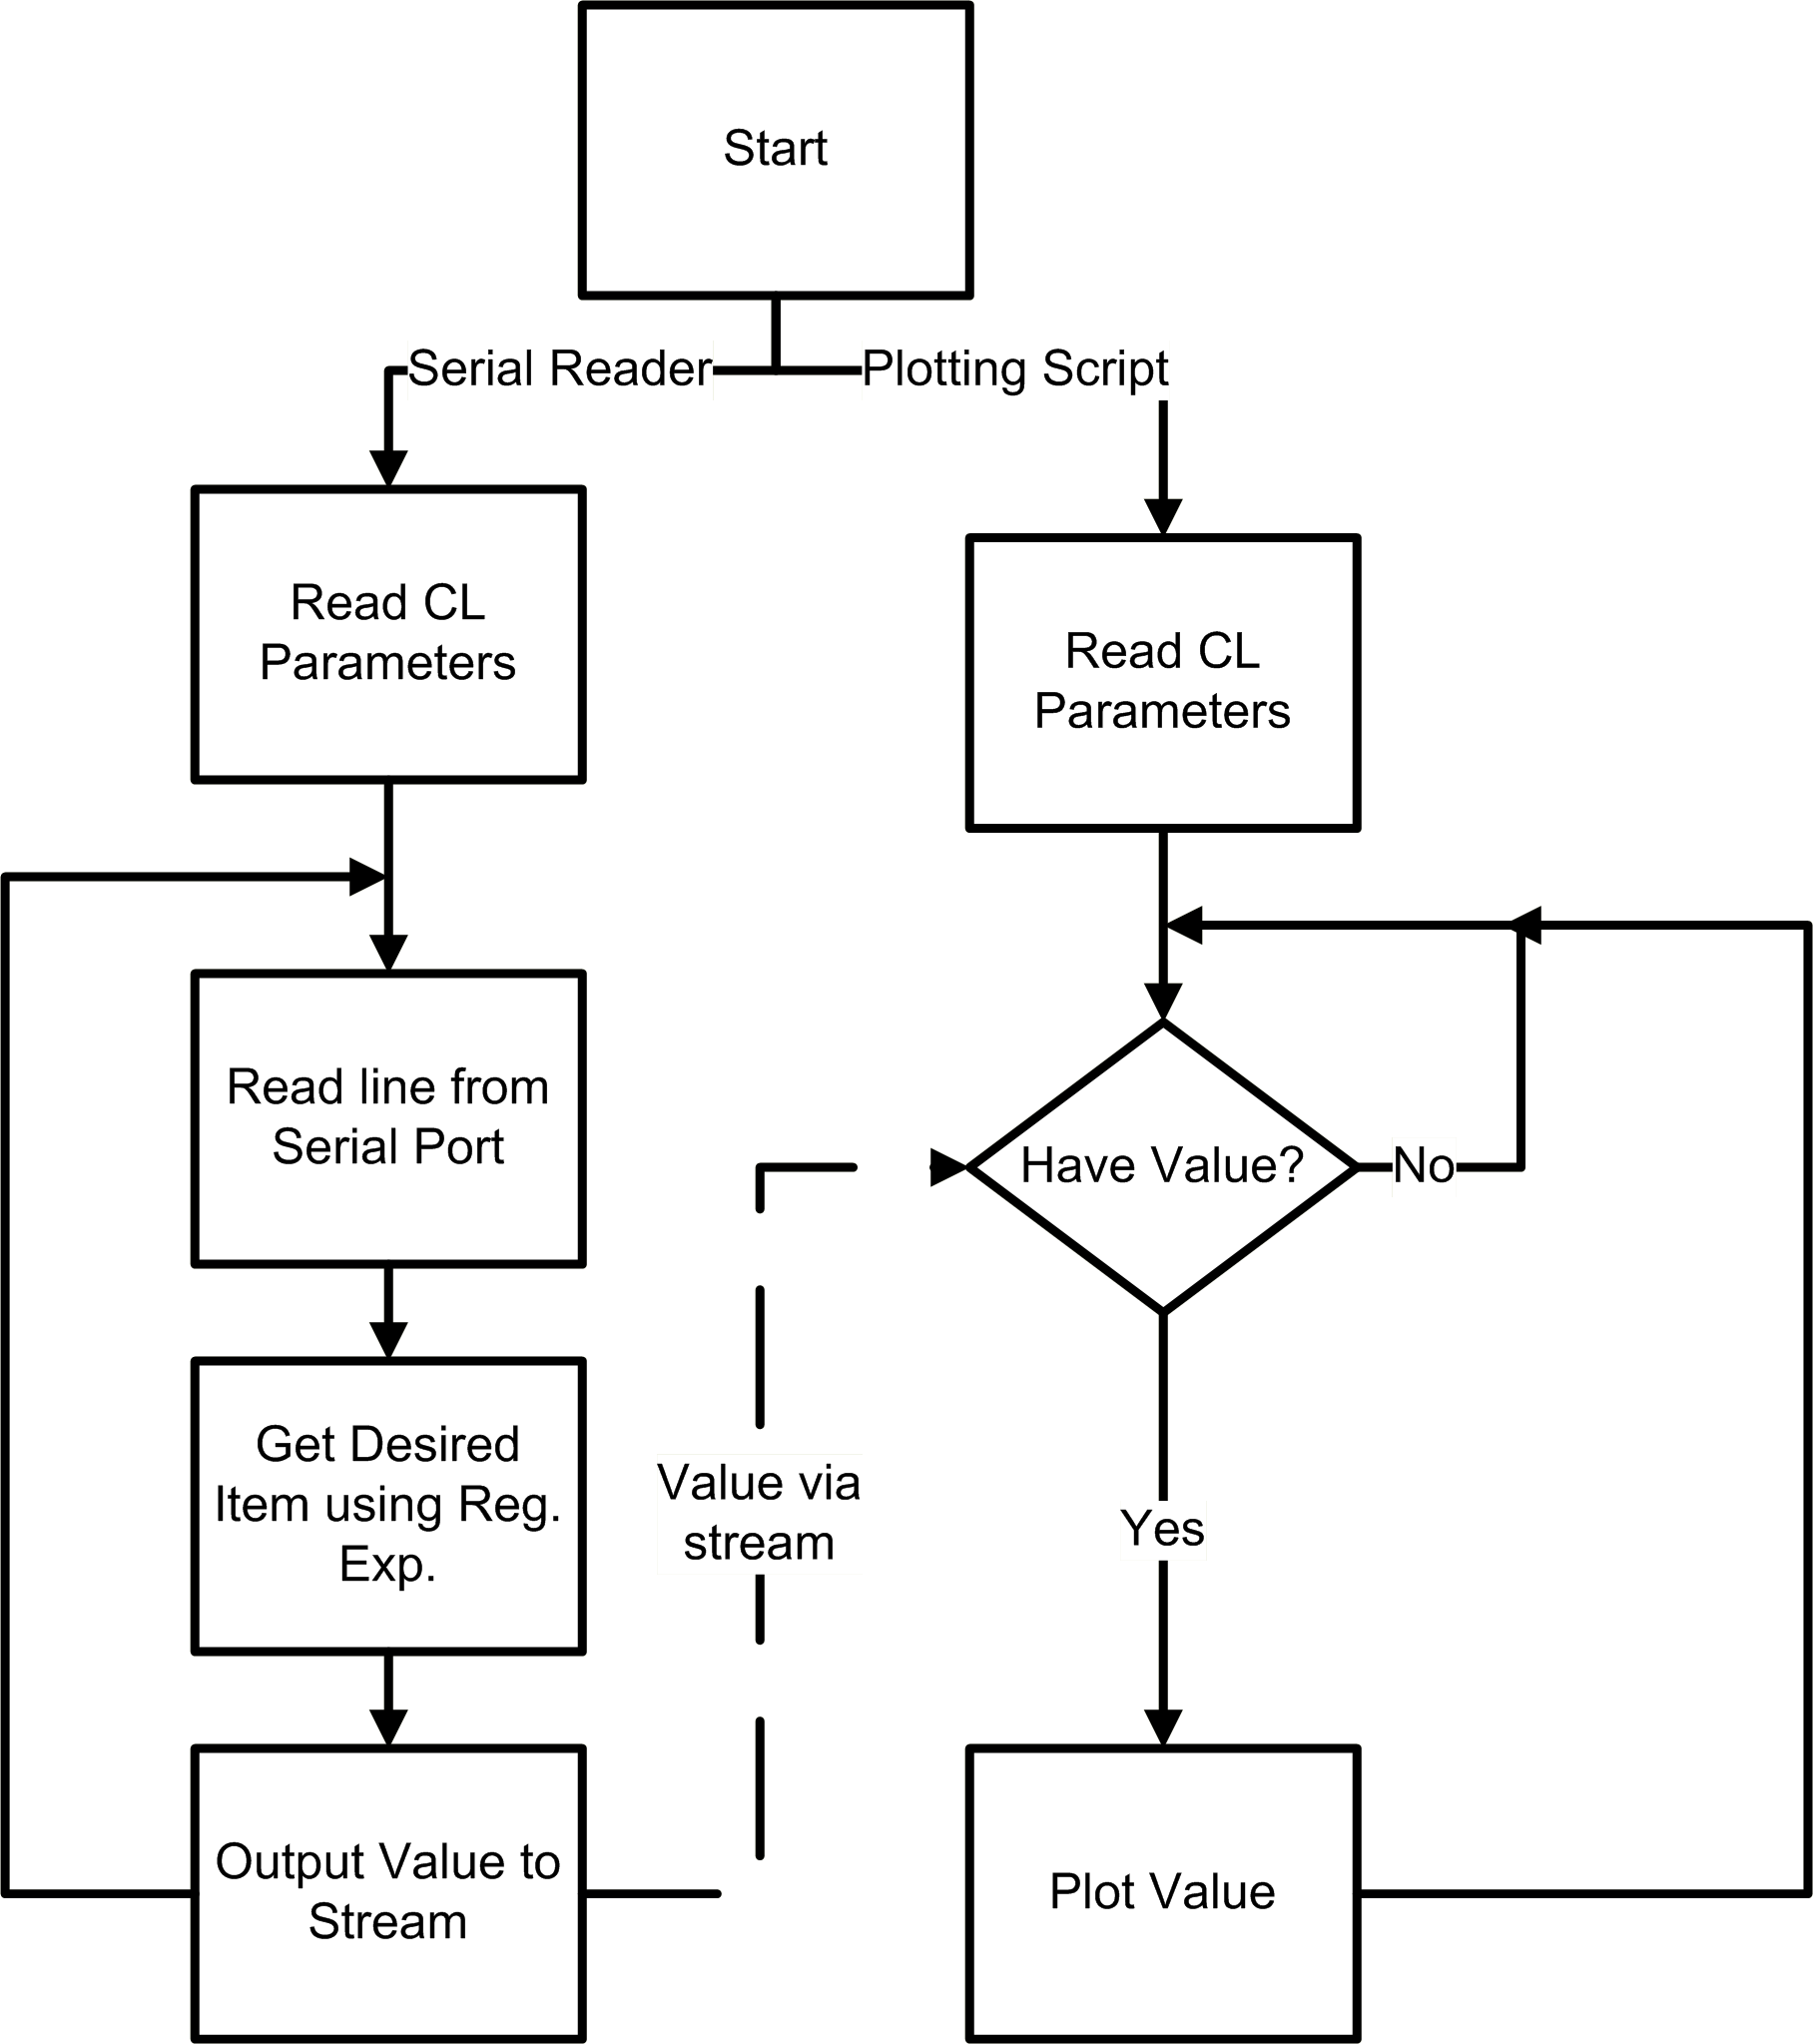
\includegraphics[width=5in]{includes/Perl_Flowchart}
    \caption{Flowchart for Perl Monitor Software}
    \label{fig:perl_flowchart}
  \end{center}
\end{figure}

The base-station software could realistically use any language that
run on a Linux machine. As is commonly known, compiled languages
typically deliver higher performance than scripted languages. C, in
particular, provides high speed and access to many low-level Linux
functions. While Perl does not have quite the speed of compiled
languages, it provides many packages to perform the desired
functions. In particular, Perl can read whole lines of input from the
serial port, use its built-in regular-expression support to select one
of several numbers and pass it as a stream into another Perl
script. Additionally, Perl scripts are portable, meaning that they can
be transferred between different machines and even different platforms
without being recompiled. The combined value of Perl's regular
expressions and portability, as well as its familiarity to the
software designer, made it a clear choice for the monitoring
program. Gnuplot provides an automatic buffer of points, aesthetically 

\subsection{Final Design}
Although the design team originally specified that a base station with
dedicated hardware would provide the best fit for the design goals and
requirements, producing a working prototype of the device proved to be too
time-consuming and difficult to debug. In place of the single-purpose
device, the design team created software to run on a Linux-based desktop
computer that can interface with the other \ac{PICA} devices.

\subsection{Testing}
In order to confirm that a hardware bases station conforms to this
design, verify each of the following. These tests confirm the general behavior,
as this should indicate that the device hardware is functioning
properly. 
\begin{enumerate}
  \item When plugged in and turned on, the base station loads its
    software and indicates this externally, such as with status
    \acp{LED}.
  \item While active, inserting a network cable will cause the base
    station to connect to the network via \ac{DHCP}. Network connectivity
    may be indicated on its own status \ac{LED}.
  \item While plugged into the network, the base station should
    display a web page when browsed by another computer on the
    network.
  \item While active, the base station should connect with other \ac{PICA}
    devices and gather their data. This should be reflected in the web
    interface.
\end{enumerate}

As the hardware will be particular to the prototype, a generic
hardware test for any base station is impractical until a prototype has
been produced. In order to verify that the development board and LEON3
processor were functioning properly, the developer took the following steps:
\begin{enumerate}
  \item Plug in the power supply and switch the board to be ``on''. If a
    change is observed, the power supply works.
  \item Verify that the on-board \ac{CPLD} is correctly programmed: the
    \acp{LED} by the directional buttons should light. If not, obtain the
    programming image from Xilinx and flash it to the \ac{CPLD} using
    \texttt{impact}. It may be located under the ML-505 board section.
  \item Verify that the networking is functioning. If a networking cable is
    inserted into the ethernet port, several status \acp{LED} along the
    front edge towards ethernet port should light or blink.
  \item Verify that the \ac{CF} port is correctly configured. Removing the
    \ac{CF} card should cause some red error \acp{LED} to light; inserting
    the card should clear them.
  \item Program the \ac{FPGA} using a bitfile. The status \acp{LED} should
    turn off during the flashing process, then turn back on
    afterwards. This process typically turns on one of the red \acp{LED}.
  \item Close \texttt{impact} and start \texttt{grmon} using the Xilinx
    \ac{USB} programmer pod. The red \ac{LED} should clear, and the console
    should reply with a readout of all the elements of system.
\end{enumerate}
Note that the \ac{FPGA} heats significantly while programmed as a LEON3. A
heatsink is not included, so caution must be exercised to avoid burns. The
likelihood of heat damage to the processor is low, as it has been run for
several hours at a time without measurable effects on performance. A
production model must deal with heat, as it will be kept on for much longer
than it would be for testing purposes.

\subsection{Future Work}
The difficulties with the hardware base station can likely be overcome with
more dedicated time and effort. If this not the case, the LEON3 system may
need to be abandoned in favor of another processor. This may require a
complete restart of this subsystem design if the error lies with the LEON3
processor. If this is the case, much of this hardware prototype design must
be revised. Concept drawings for the web interface may be seen in figures
\ref{fig:ui_mockup_history} and \ref{fig:ui_mockup_localized}.

\begin{figure}[htbp]
  \begin{center}
  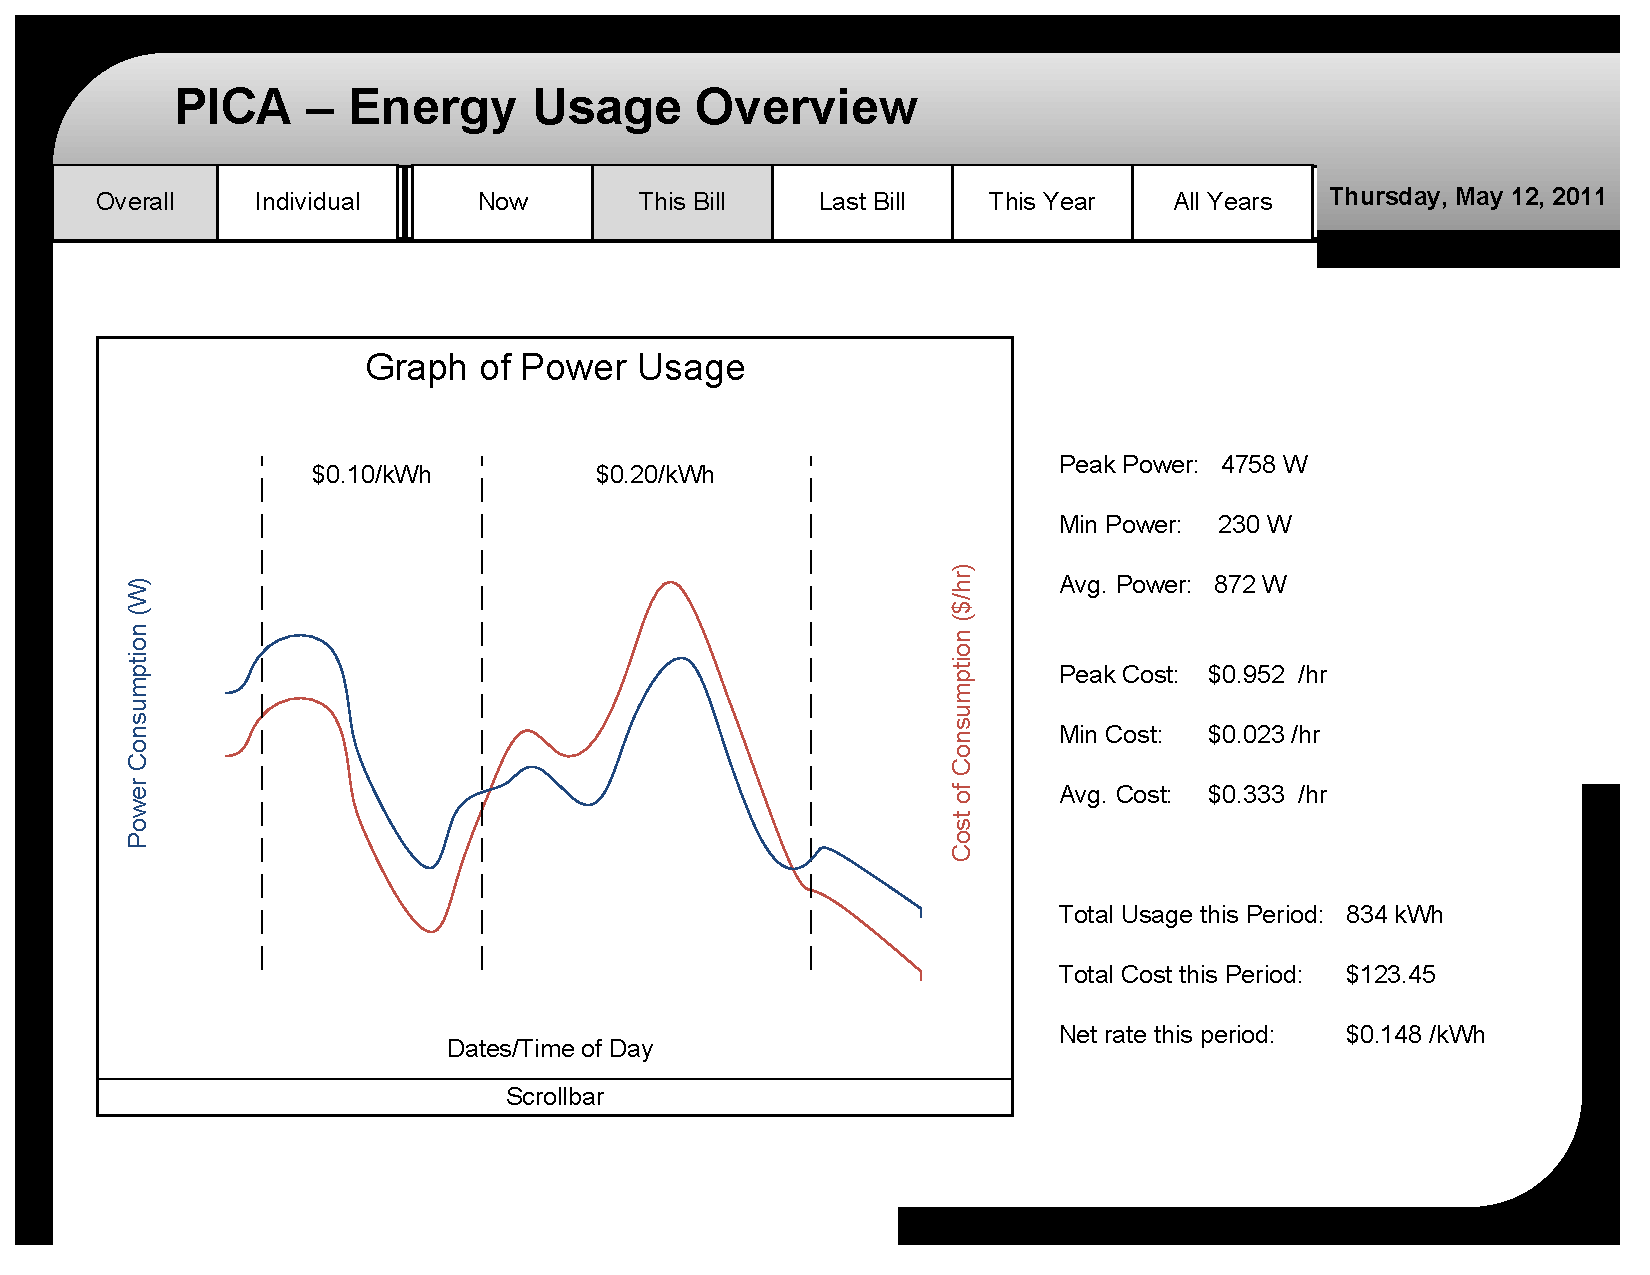
\includegraphics[angle=90,width=6.5in]{includes/base_ui_mockup_recent}
  \caption{Conceptual Base-Station Interface: Power History}
  \label{fig:ui_mockup_history}
\end{center}
\end{figure}


\begin{figure}[htbp]
  \begin{center}
  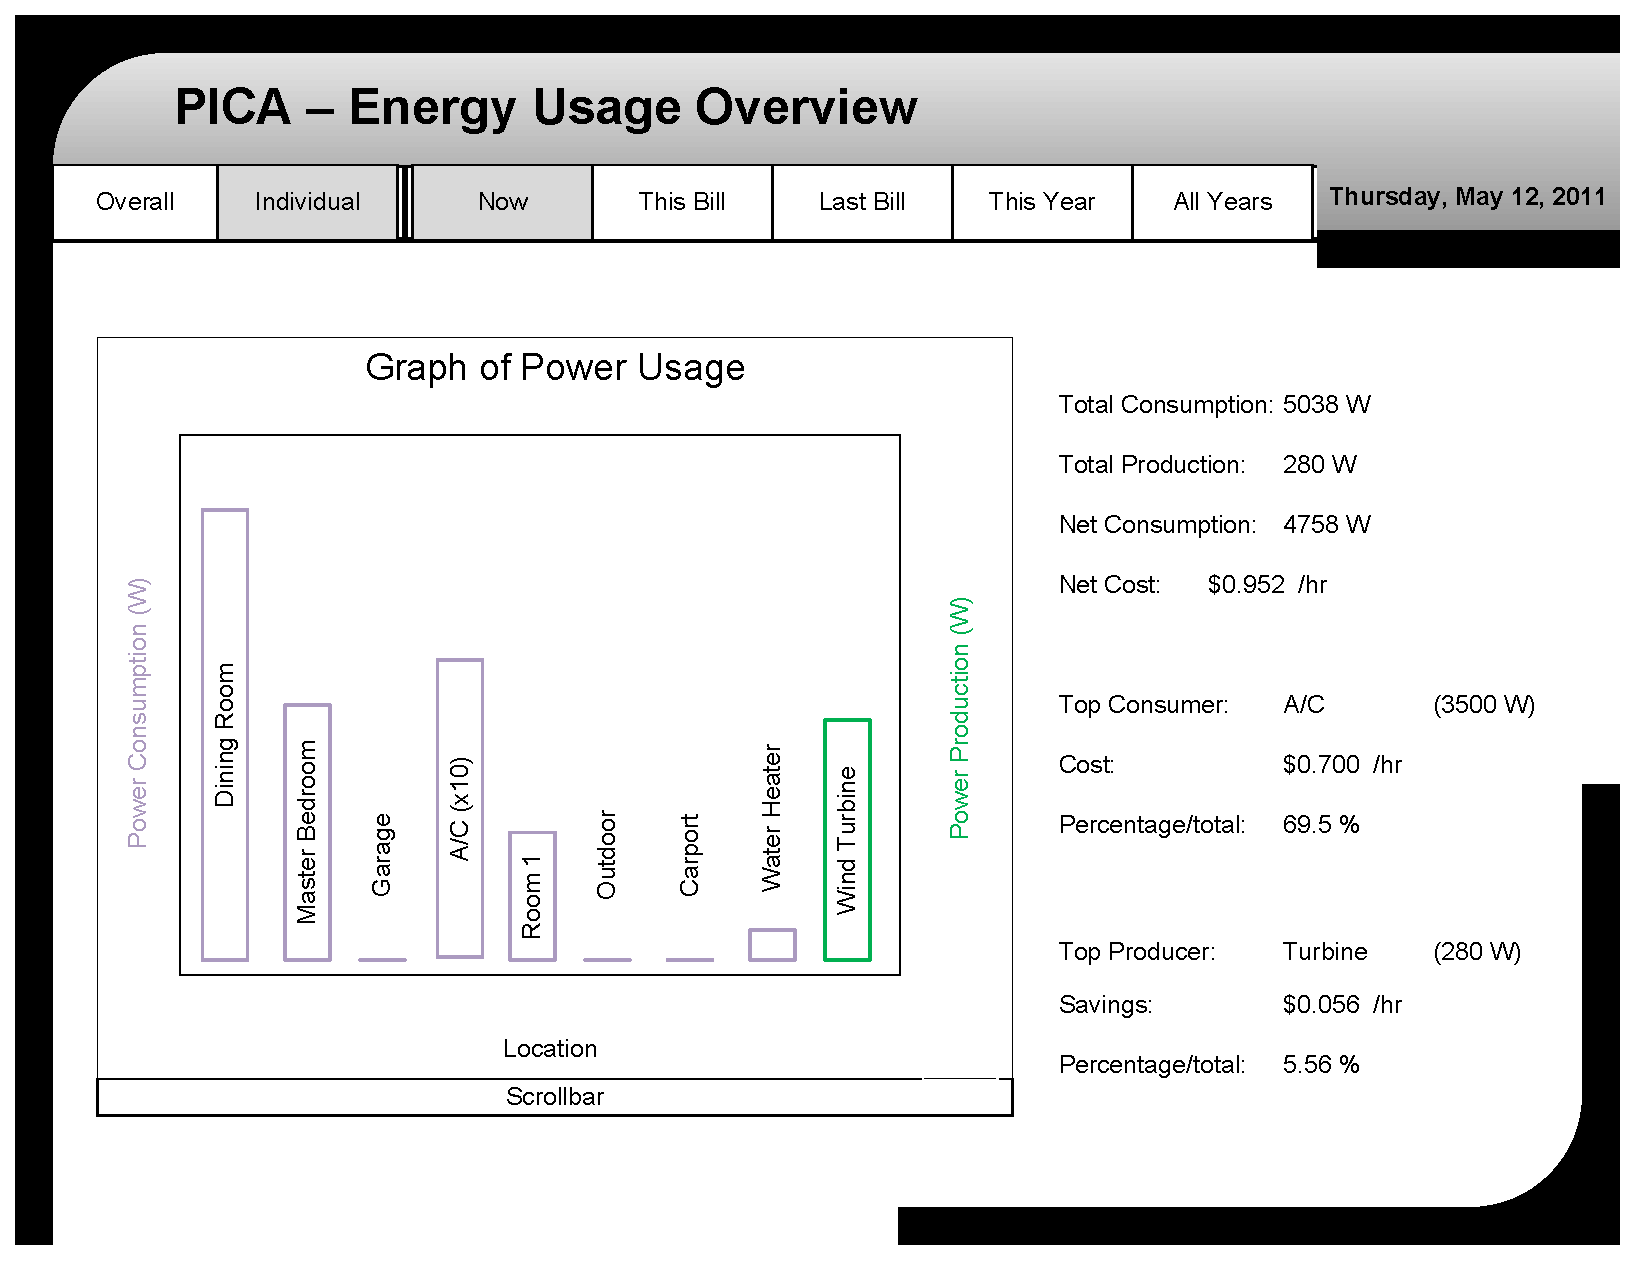
\includegraphics[angle=90,width=6.5in]{includes/base_ui_mockup_multiple}
  \caption{Conceptual Base-Station Interface: Localized Measurements}
  \label{fig:ui_mockup_localized}
\end{center}
\end{figure}


\subsubsection{Software Monitor}
The software monitor lacks several features intended for the original
base station. Adding them to the Perl scripts would provide a good
hold-over in the absence of a hardware base station. In fact, a
hardware base station could use some components of the Perl scripts if Perl
is installed on the base station.
\begin{enumerate}
  \item Allow data to be backed up to a file.
  \item Read data from a backup file and display information about it.
  \item When supported, instruct connected systems to change their
    output.
  \item Provide a way to restrain all devices from talking at once.
  \item Distinguish devices from each other.
  \item Support data encryption and decryption between devices.
\end{enumerate}